\chapter{\IfLanguageName{dutch}{Resultaten}{Results}}%
\label{ch:resultaten}

In dit hoofdstuk worden de resultaten uit de requirementsanalyse, vergelijkende studie en de ontwikkeling van het prototype besproken. 

\section{Requirementsanalyse}

ChatGPT en Bing Chat zijn capabel om alle lexicale en syntactische vereenvoudigingstechnieken te realiseren. Tools, buiten Bing Chat en ChatGPT, zijn niet in staat om een formaatwijziging toe te passen. Enkel MTS is hiertoe voorlopig in staat, maar ChatGPT en Bing Chat maken gebruik van een technisch capabel taalmodel die deze taak kan realiseren. Het achterliggende taalmodel van beide tools is online via API beschikbaar. Daarmee is het aanbieden van gepersonaliseerde tekstvereenvoudiging bestaande uit lexicale, syntactische en structurele aanpassingen een \textit{must-have} voor prototype. Zoals uitgewezen in de literatuurstudie zijn er Python-libraries die dit realiseren, en daarmee vormt deze taak eveneens als een \textit{must-have} voor het prototype. Geen uitgeteste tool maakt gebruik van een personaliseerbare website. Daarop nog maken de uitgeteste sites weinig gebruik van de aangeraden aanschouwelijkheidsopties weergegeven in tabel \ref{table:dyslexia-necessaries}. Het prototype kan hiermee uitpakken en daarom vormt de personaliseerbare site als een \textit{must-have} voor het prototype. Om de tool te kunnen doorgeven aan vakexperten, wordt het prototype ook ontworpen met een lokale opzet in gedachten. Tools zoals Docker kunnen dit realiseren. Alle tools, buiten ChatGPT en Bing Chat, zijn in staat om een PDF met de vereenvoudigde tekstinhoud te genereren.

\medspace

Zowel Kurzweil3000 als Simplish bieden gegenereerde woordenlijsten aan, na de handmatige selectie van de gebruiker. Deze toevoeging is eerder ondersteunend, zoals aangewezen in tabel \ref{table:benefits-mts}. Daardoor is deze taak een \textit{should-have} voor het prototype. Zoals eerder aangehaald zijn tools in staat om een PDF te genereren, maar deze output is noch gepersonaliseerd noch heeft de eindgebruiker inbreng op hoe de uitvoer eruit moet zien. Open-sourcepakketten maken dit haalbaar en daarmee vormt deze taak een \textit{should-have}.

\medspace

Enkel Simplish en Rewordify bieden een ingebouwde tekstanalysemodele aan, zoals weergegeven in figuren \ref{img:simplish-output} en \ref{img:scholarcy}. Andere tools beschikken over geen leesgraadsmetrieken, noch van het ingegeven document, noch van het vereenvoudigde document. Simplish maakt gebruik van kleurcodecriteria om meer transparantie aan te reiken over de getransformeerde tekst, waaronder niet-veranderende woorden, adequate vertalingen, uitleg naar de voetnoot, homoniemen of woorden die geen eenvoudigere synoniemen hebben. Zoals aangegeven in figuur \ref{img:simplish-output} duidt de vergelijkende weergave de verschillen aan tussen de oorspronkelijke en vereenvoudigde tekst. Simplish beklemtoont de transformaties door middel van kleurcodes. Rewordify vult hierop aan en biedt meer inzichten in de leesbaarheidsgraad van de vereenvoudigde tekst, zoals geïllustreerd in figuur \ref{img:scholarcy}. Experimenten met Simplish en Rewordify wijzen uit dat dit een haalbare taak is, maar deze taak behoort niet tot prioriteit van het prototype en is daarmee een \textit{could-have}. Geen tool maakt gebruik van automatische selectie van moeilijke woorden, buiten ChatGPT en Bing Chat die dit enkel kunnen doen na een expliciete commando. ChatGPT en Bing Chat wijzen uit dat dit een haalbare taak is, mits het gebruik van een expliciete prompt, en daarom vormt deze taak een \textit{could-have} voor het prototype.

\medspace

De uitgeteste tools zijn allemaal online beschikbaar. Toch is dit onderzoek te kleinschalig om een volledig online beschikbare webtoepassing waar te maken en wordt deze taak als een \textit{wont-have} ingeschat. Daarmee blijft de opzet van de webtoepassing binnen een lokale omgeving. Ten slotte zijn de gebruikte tools of taalmodellen niet mogelijk binnen een lokale opzet. Zo is het GPT-3 model te groot om op een laptop lokaal te doen draaien. Daarom is de lokale hosting van het taalmodel een \textit{wont-have} voor het prototype. 

\section{Vergelijkende studie}

Na een tekstvereenvoudiging ligt het aantal zinnen bij T1, T2 en T3 hoger dan dat van de oorspronkelijke tekst. Elke prompt van T4 maakt gebruik van meer zinnen dan het oorspronkelijk artikel, zoals aangewezen in tabel \ref{table:resultaten-aantal-woorden}.

\begin{table}[h]
	\centering
	\begin{tabular}{ | m{3cm} | m{3cm} | m{3cm} | } 
		\hline
		Bron & #Zinnen in A1 & #Zinnen in A2 \\
		\hline
		Oorspronkelijk & 78  & 159 \\ 
		\hline
		MTS (door leerkracht) & 43 & 45 \\
		\hline
		MTS (door leerling) & n.v.t. & 50 \\
		\hline
		T1 & 101 & 209 \\
		\hline
		T2 & 82 & 209 \\
		\hline
		T3 & 100 & 209 \\
		\hline
		T4 P1 & 61 & 98 \\
		\hline
		T4 P2 & 89 & 133 \\
		\hline
		T4 P3 & 39 & 55 \\
		\hline
	\end{tabular}
	\label{table:resultaten-aantal-woorden}
	\caption{Aantal zinnen per }
\end{table}

T1, T2 en T3 gebruiken gemiddeld minder woorden per zin dan het oorspronkelijk artikel. Enkel P3 is in staat om gemiddeld minder woorden per zin te gebruiken, vergeleken met P1 en P2 die elk gemiddeld meer dan 19 woorden per zin gebruiken, zoals aangegeven in figuren \ref{img:boxplot-min-max-avg-words-a1} en \ref{img:boxplot-min-max-avg-words-a2}.

\begin{figure}
	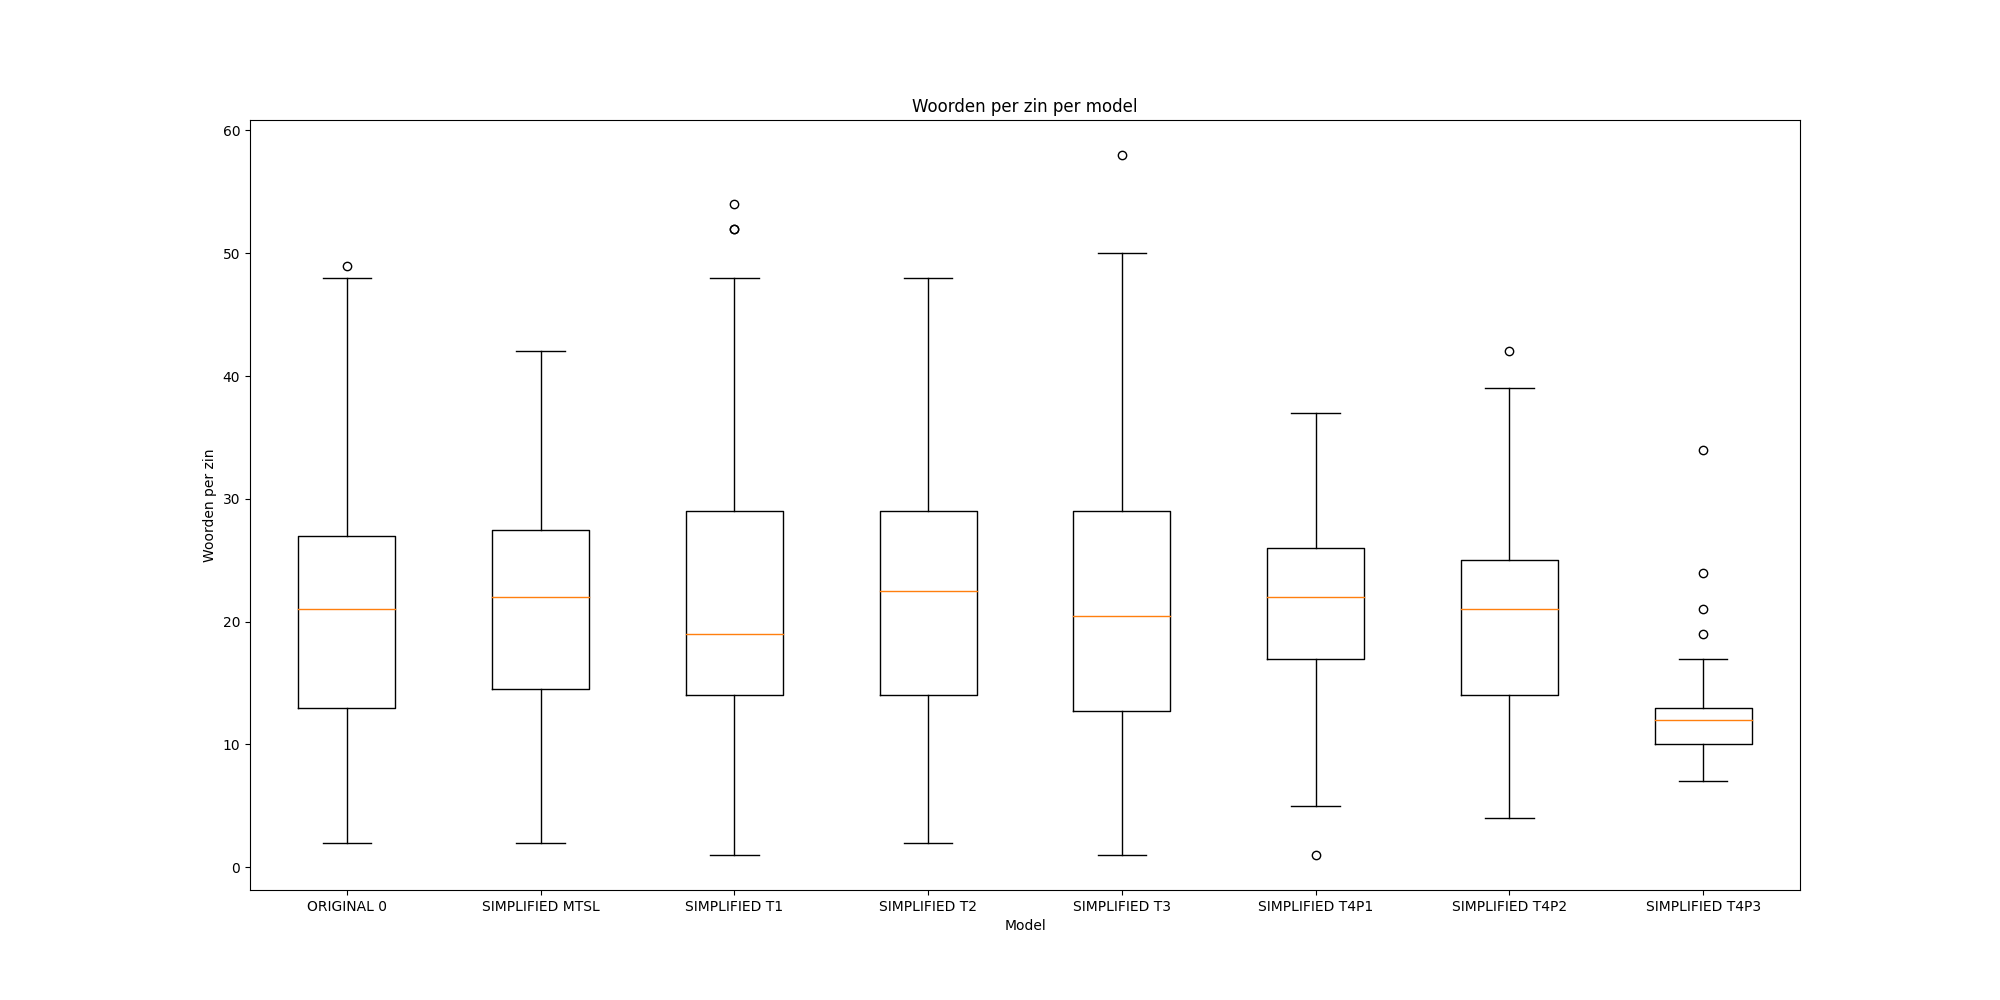
\includegraphics[width=\linewidth]{img/boxplot-avg-a1.png}
	\caption{Overzicht van het minimum, maximum en gemiddeld aantal woorden per zin per model in artikel 1.}
	\label{img:boxplot-min-max-avg-words-a1}
\end{figure}

\begin{figure}
	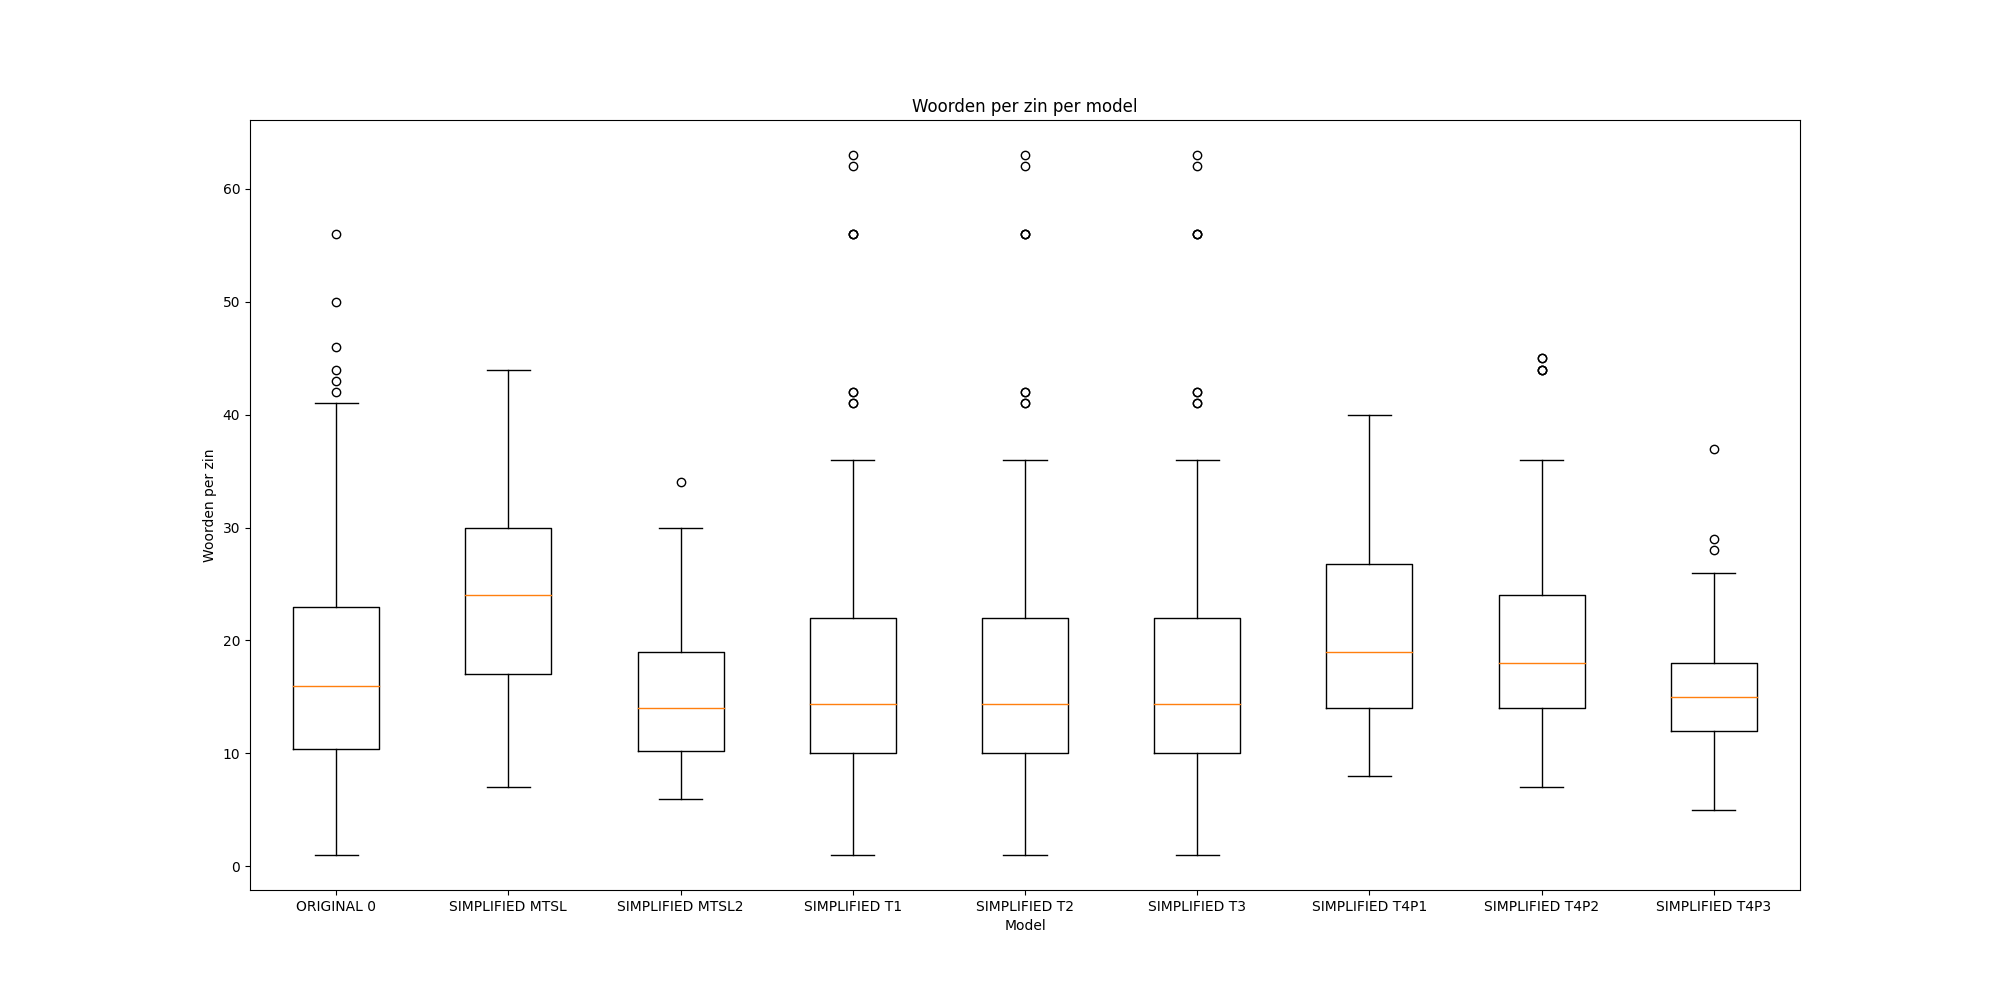
\includegraphics[width=\linewidth]{img/boxplot-avg-a2.png}
	\caption{Overzicht van het minimum, maximum en gemiddeld aantal woorden per zin per model in artikel 2.}
	\label{img:boxplot-min-max-avg-words-a2}
\end{figure}

\medspace

De FRE-scores bij alle geteste taalmodellen en MTS-referentieteksten zijn niet significant hoger of lager, vergeleken met het oorspronkelijk wetenschappelijk artikel, zoals aangetoond in figuren \ref{img:boxplot-fre-a1} en \ref{img:boxplot-fre-a2}. Eveneens zijn de FOG-scores ook niet significant hoger of lager bij de vereenvoudigde wetenschappelijke artikelen zoals aangewezen in \ref{img:boxplot-fog-a1}, \ref{img:boxplot-fog-a2}.

\begin{figure}
	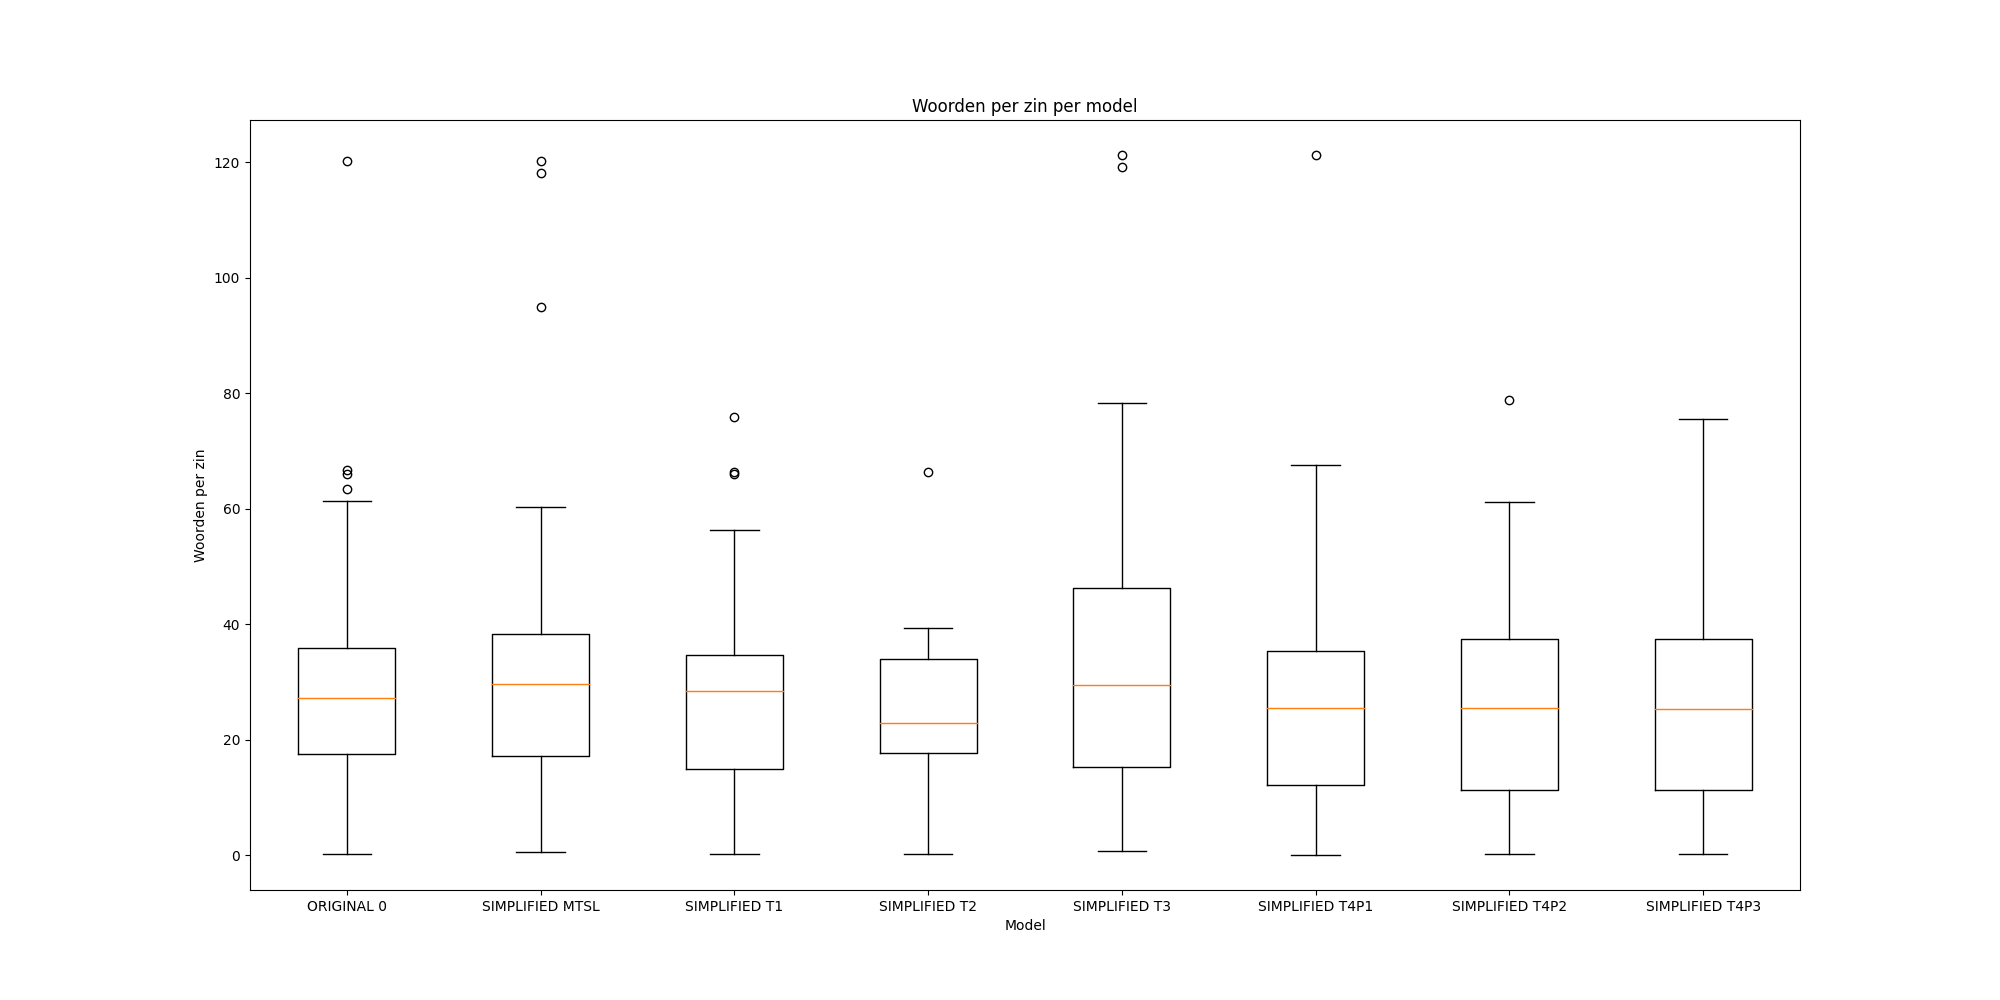
\includegraphics[width=\linewidth]{img/boxplot-fre-a1.png}
	\caption{Boxplot van de FRE-scores voor A1.}
	\label{img:boxplot-fre-a1}
\end{figure}

\begin{figure}
	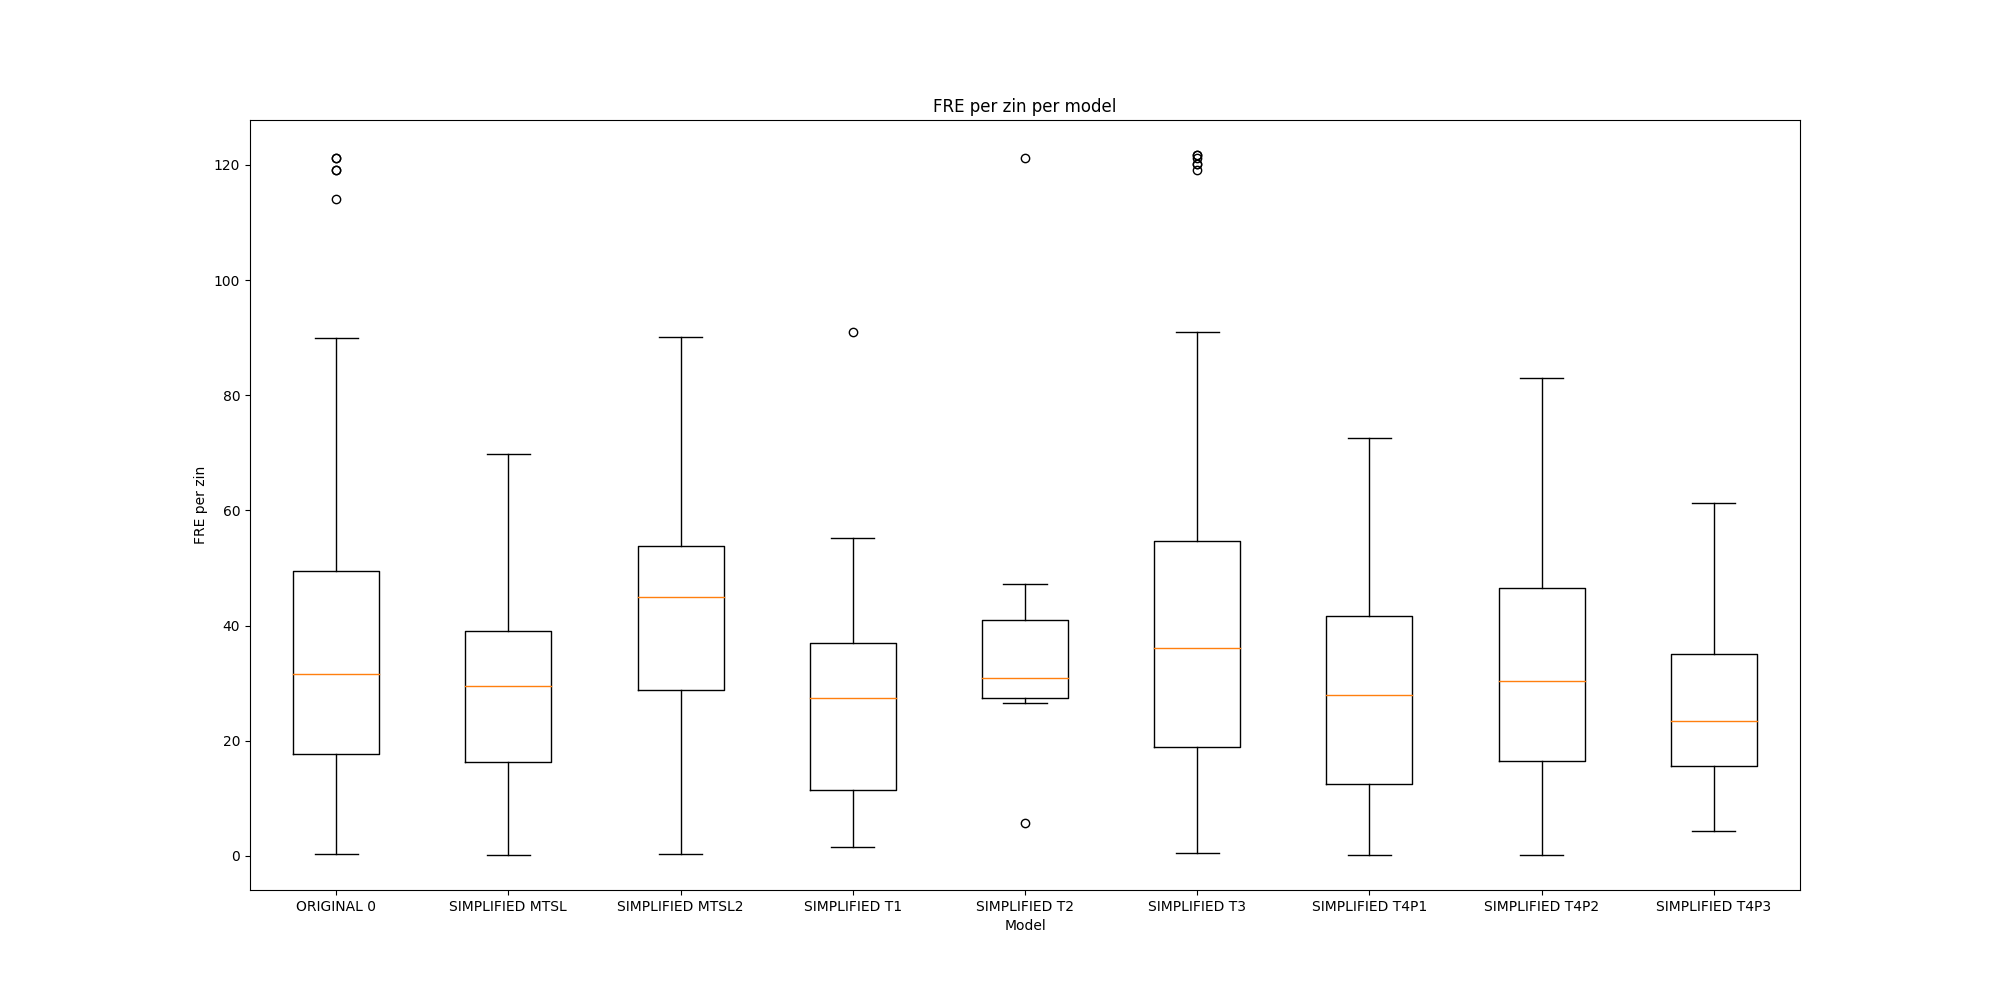
\includegraphics[width=\linewidth]{img/boxplot-fre-a2.png}
	\caption{Boxplot van de FRE-scores voor A2.}
	\label{img:boxplot-fre-a2}
\end{figure}

\begin{figure}
	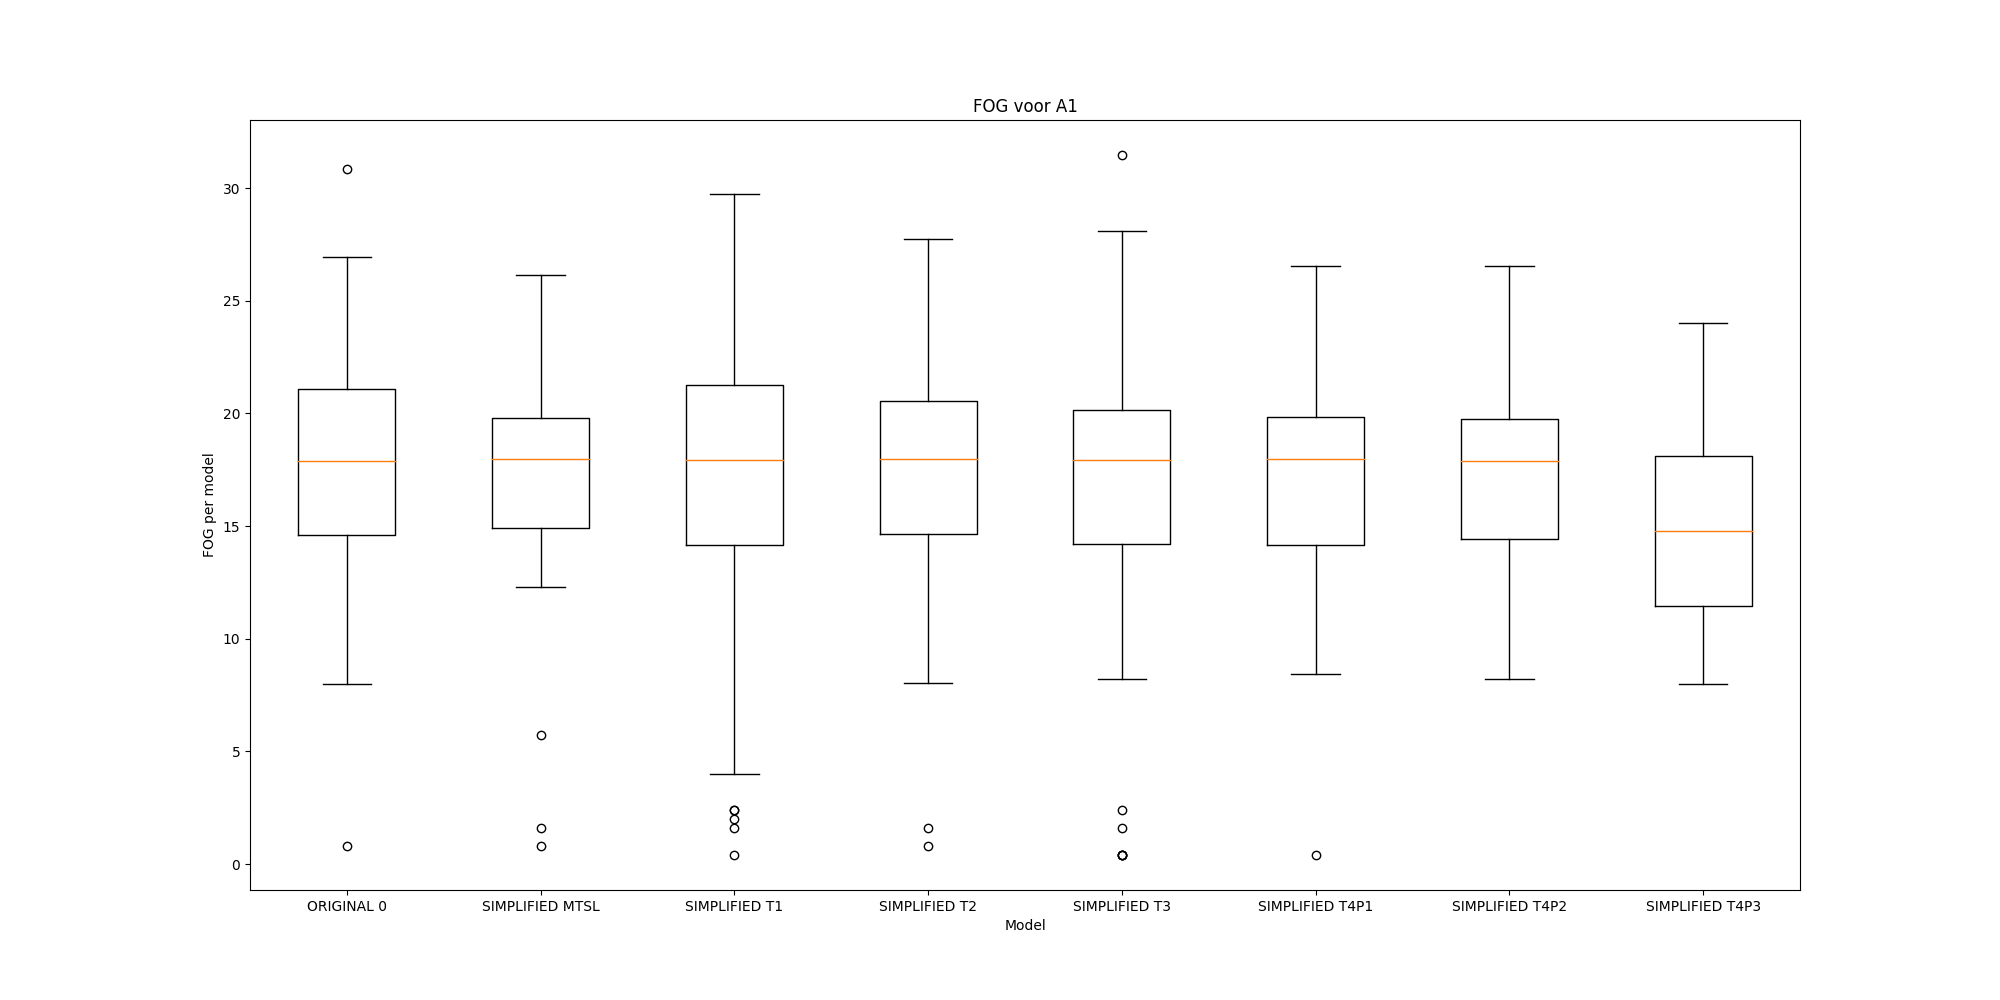
\includegraphics[width=\linewidth]{img/boxplot-fog-a1.png}
	\caption{Boxplot van de FOG-scores voor A1.}
	\label{img:boxplot-fog-a1}
\end{figure}

\begin{figure}
	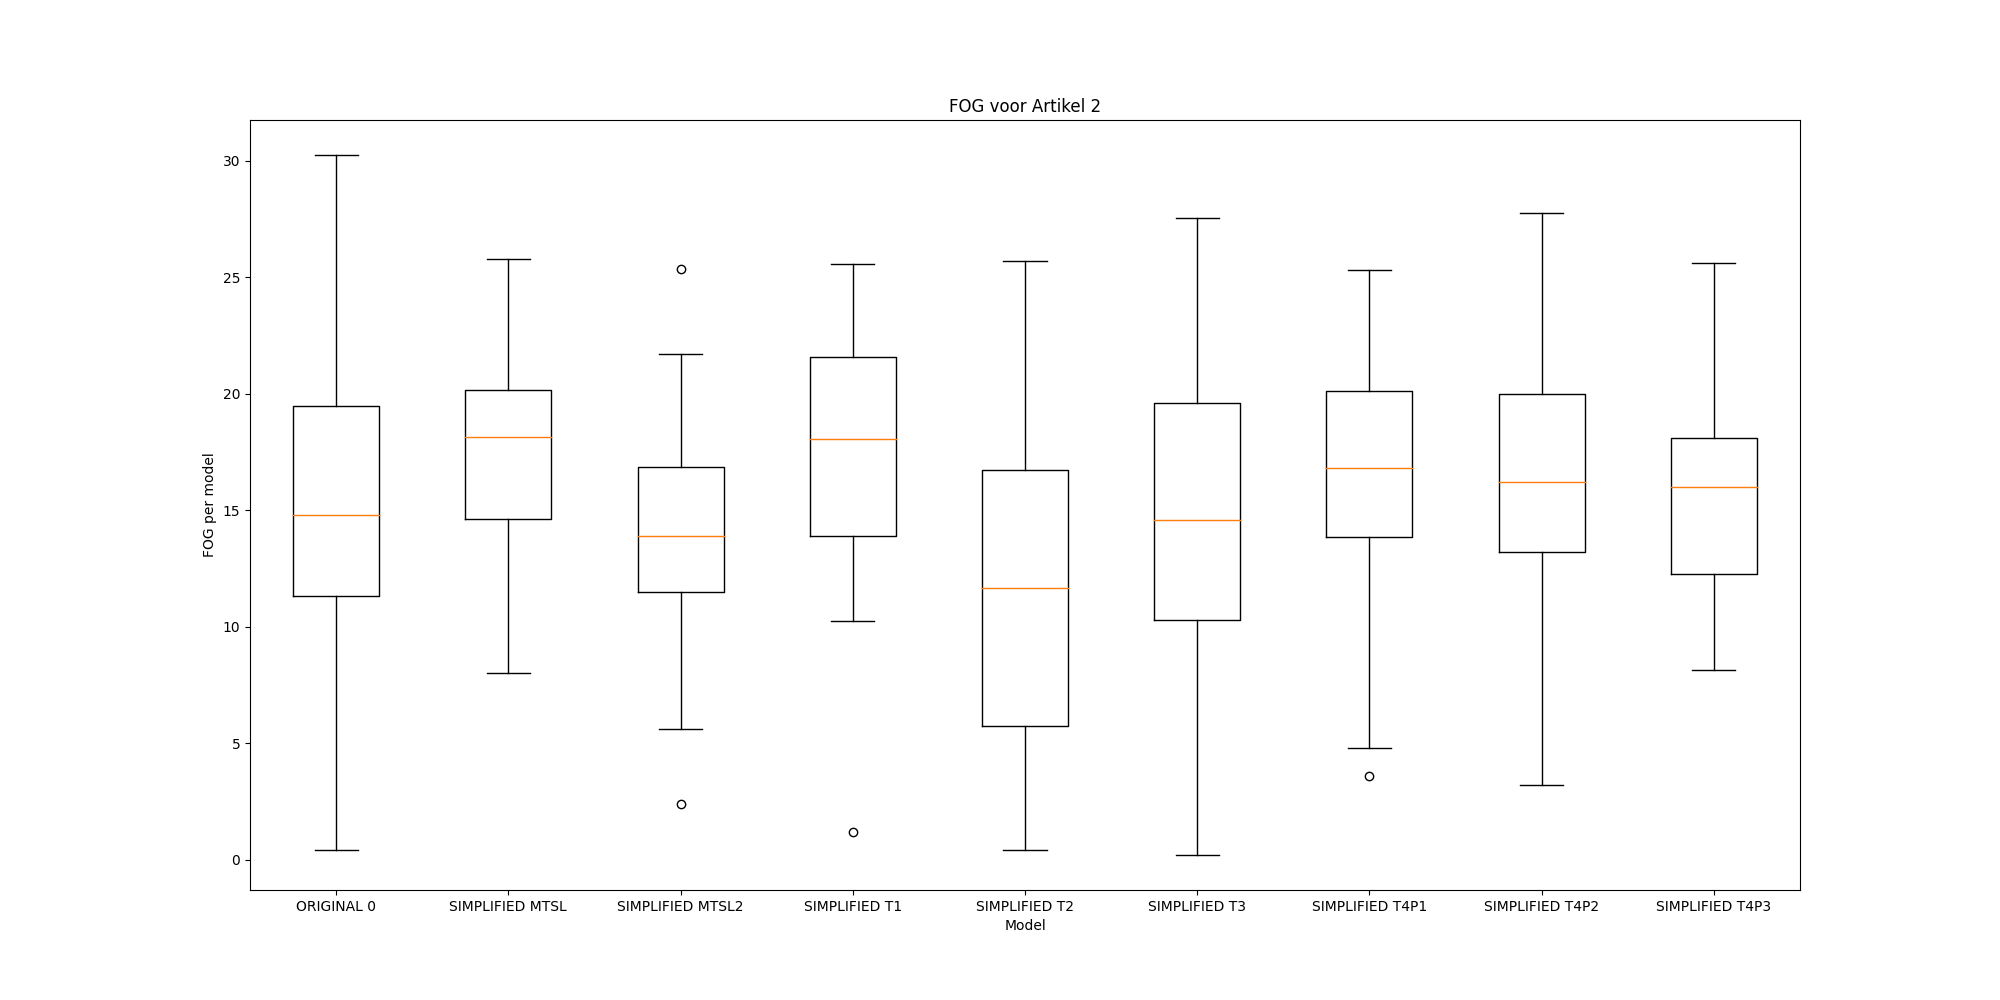
\includegraphics[width=\linewidth]{img/boxplot-fog-a2.png}
	\caption{Boxplot van de FOG-scores voor A2.}
	\label{img:boxplot-fog-a2}
\end{figure}

% TODO

\begin{figure}
	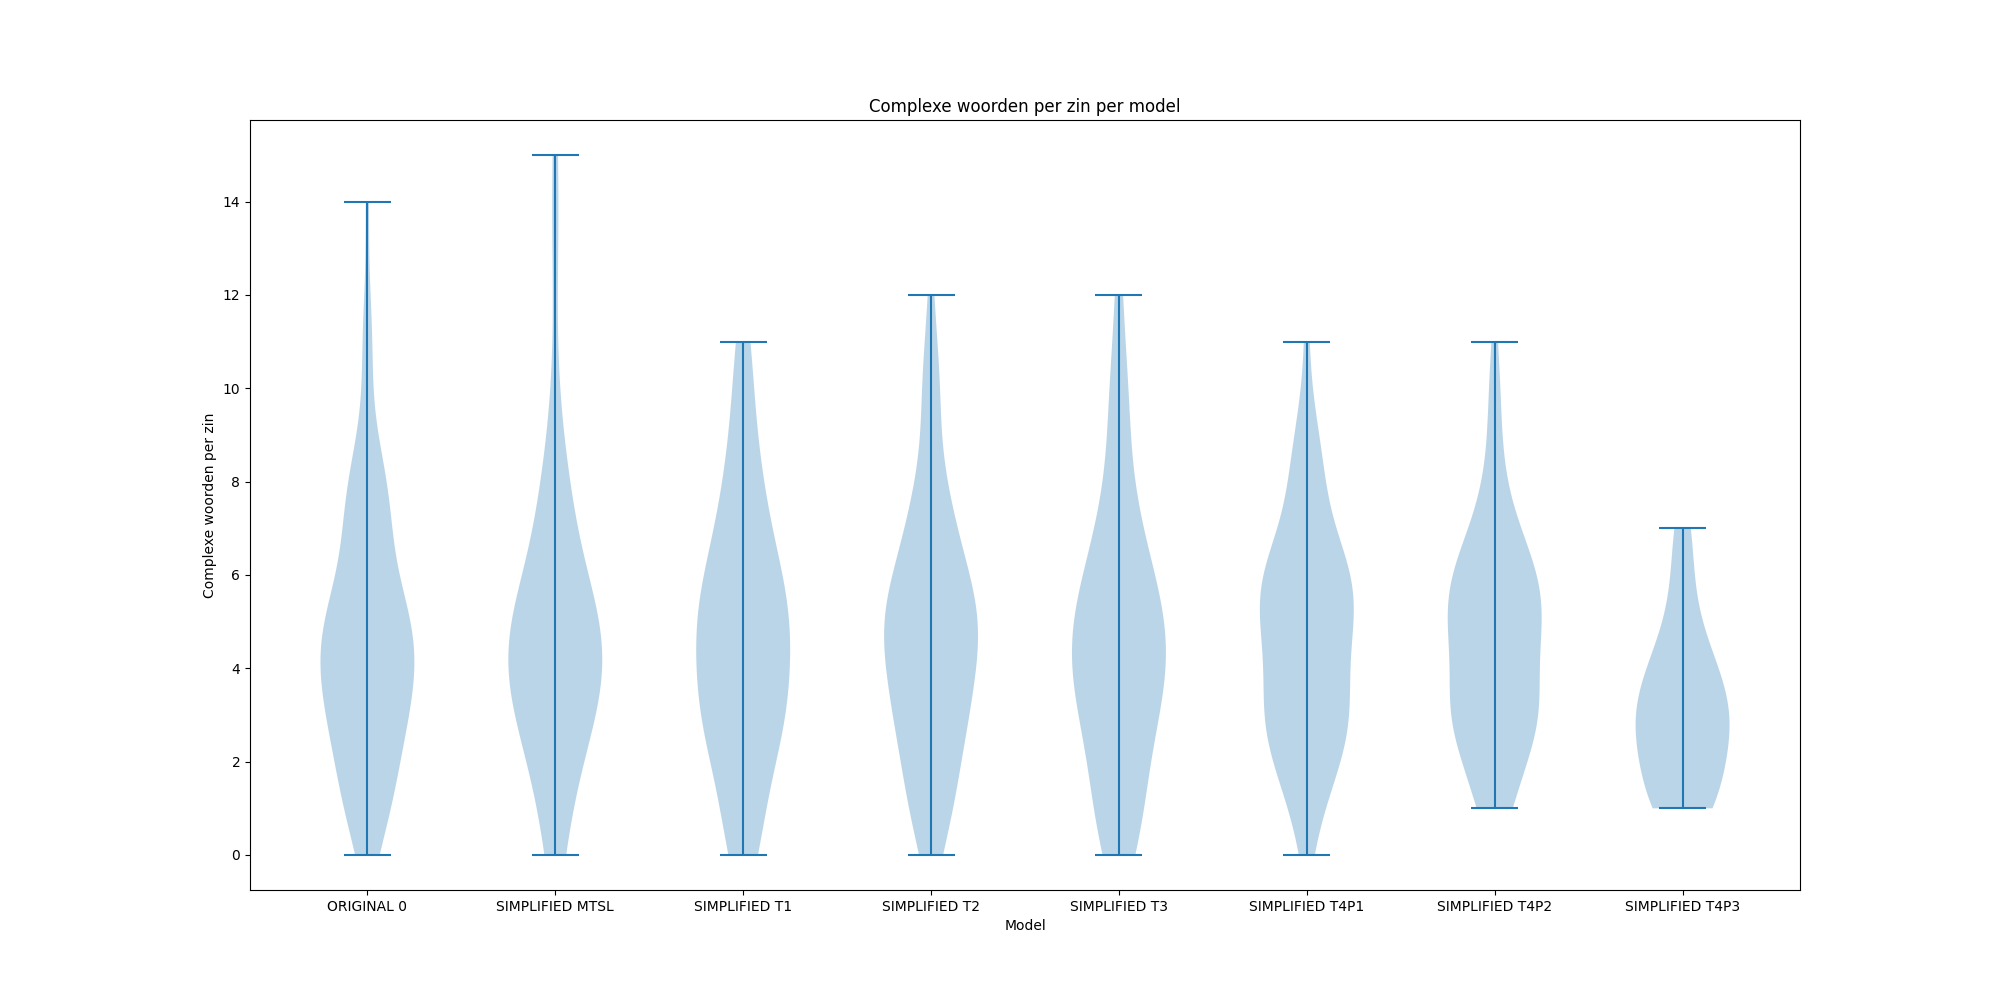
\includegraphics[width=\linewidth]{img/violinplot-complex-a1.png}
	\caption{Complexe woorden per model.}
	\label{img:violinplot-complex-a1}
\end{figure}

\begin{figure}
	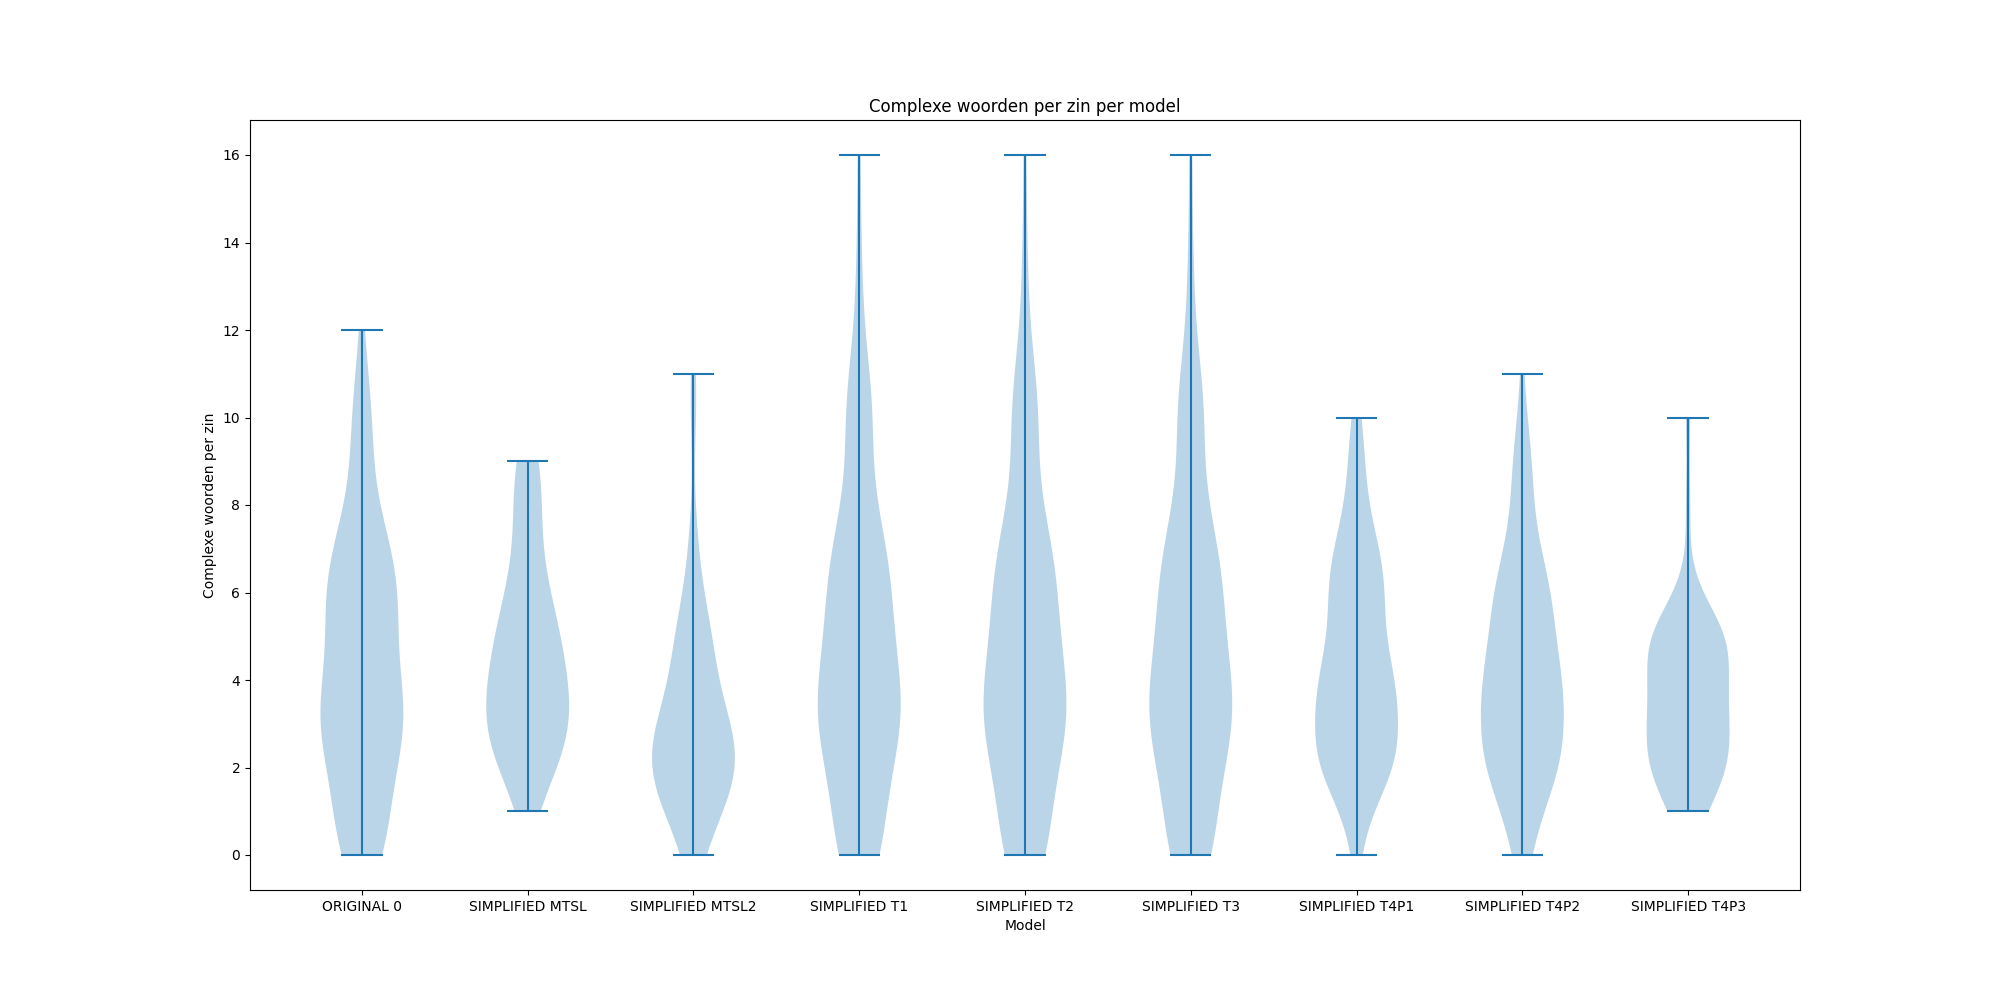
\includegraphics[width=\linewidth]{img/violinplot-complex-a2.png}
	\caption{Gemiddeld aantal complexe woorden per zin gegroepeerd op model.}
	\label{img:violinplot-complex-a2}
\end{figure}

T1, T2 en T3 maken bij A1 en A2 gebruik van langere woorden ten opzichte van de oorspronkelijke tekst, in tegen stelling tot de drie T4 prompts die wel gebruik maken van kortere woorden en zo gelijkaardige resultaten bekomen als de MTS-referentieteksten. Deze verhouding wordt aangewezen in figuren 

\begin{figure}
	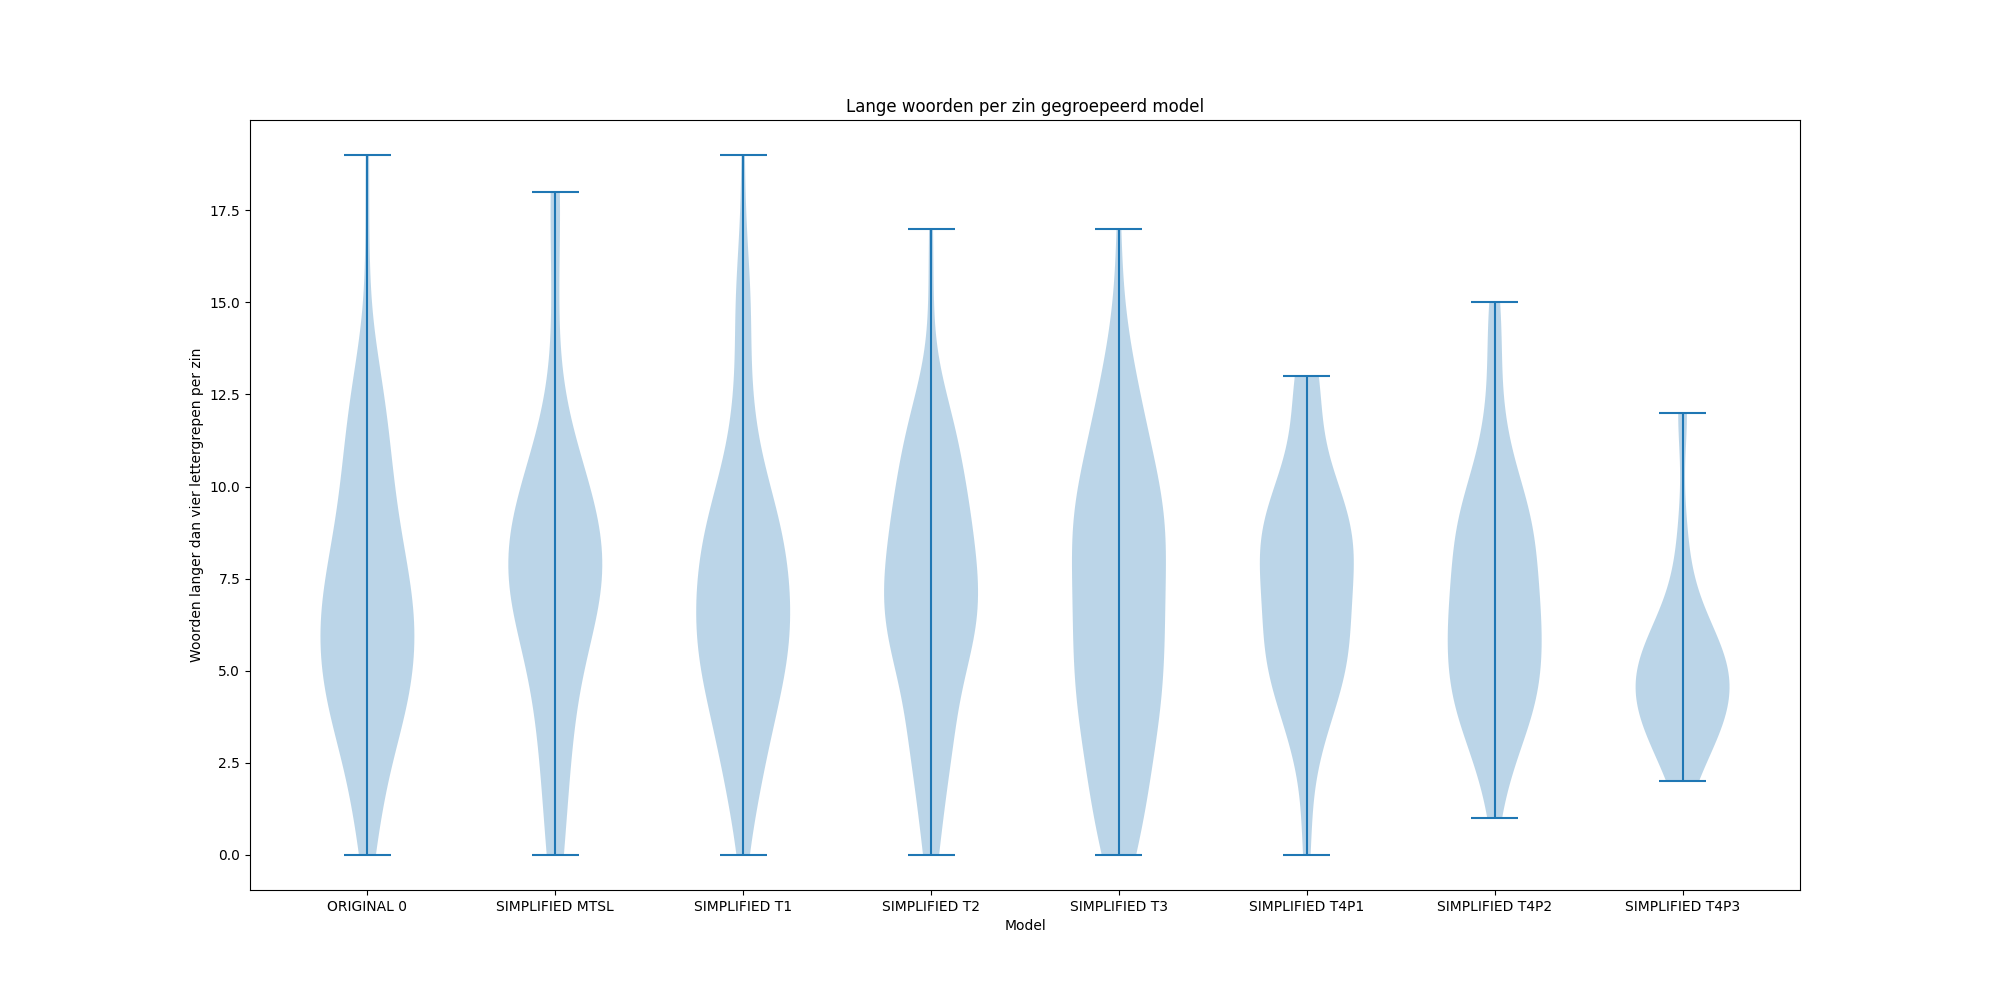
\includegraphics[width=\linewidth]{img/violinplot-long-a1.png}
	\caption{Gemiddeld aantal lange woorden per zin gegroepeerd op model.}
	\label{img:violinplot-long-a1}
\end{figure}

\begin{figure}
	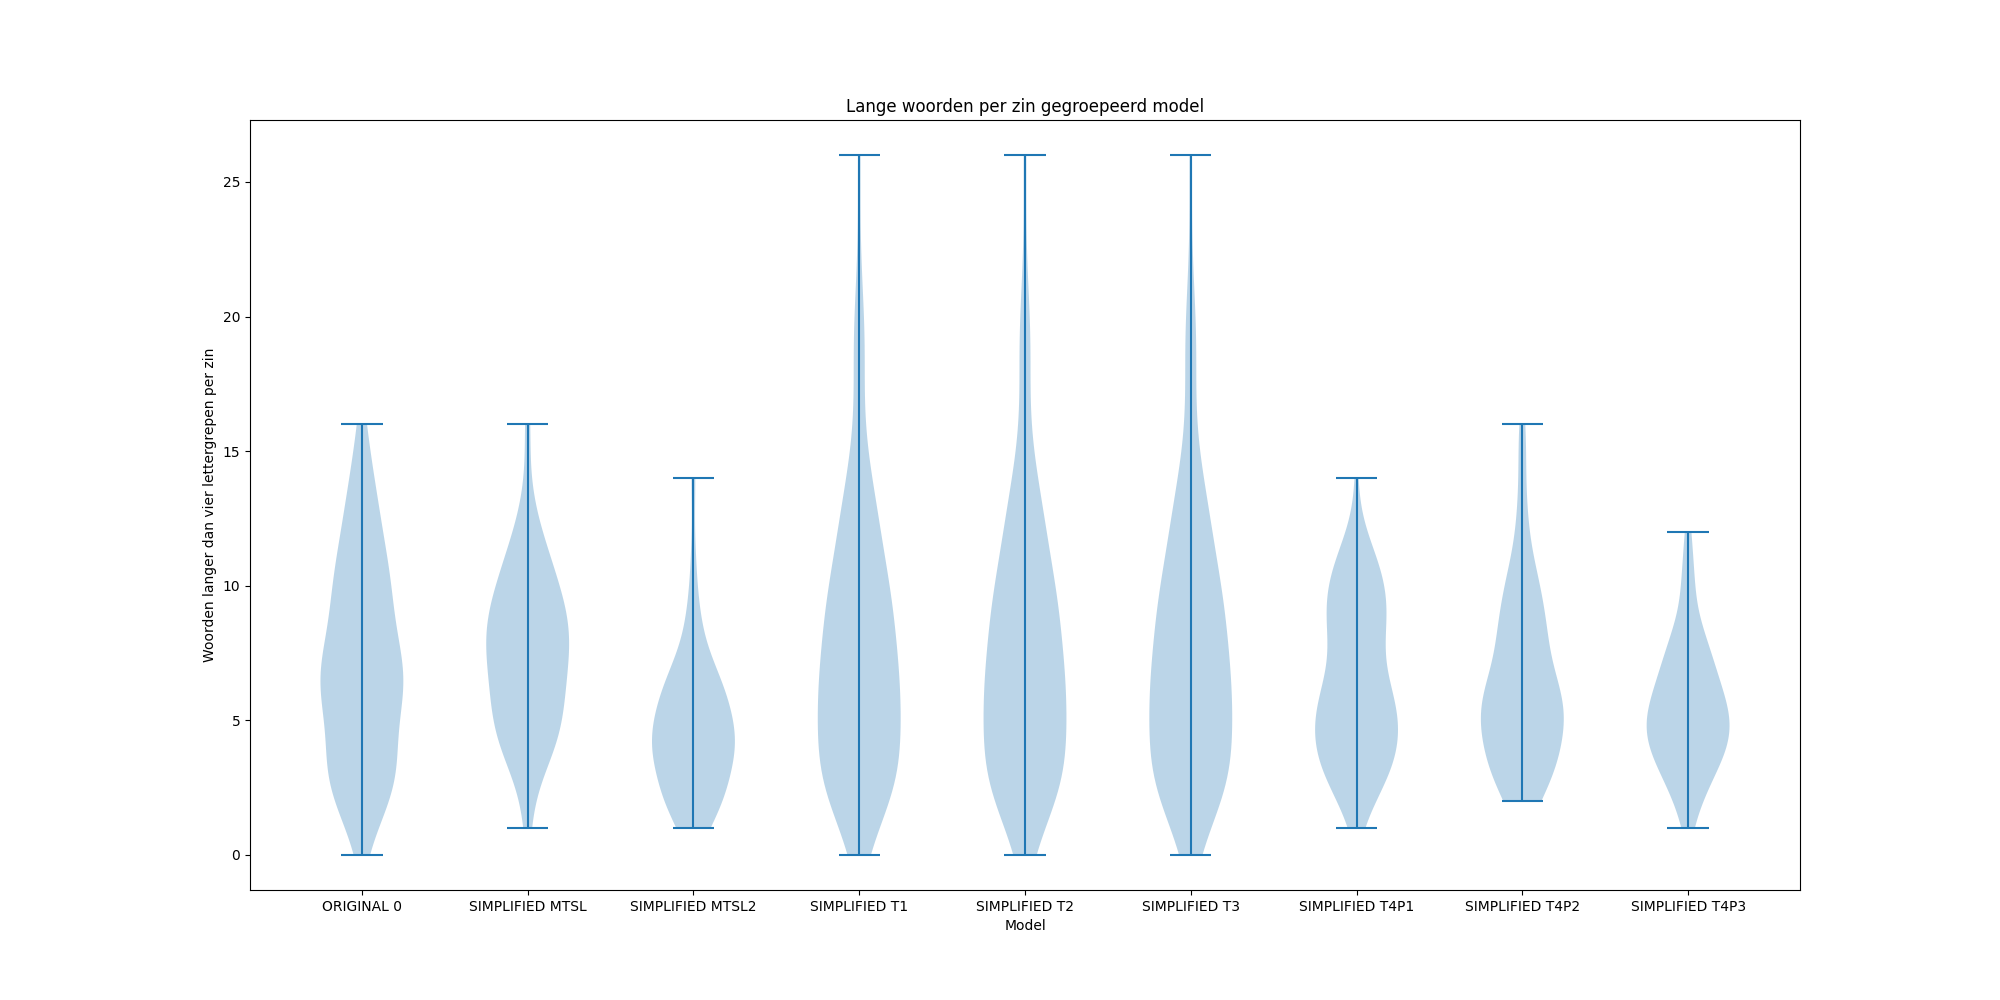
\includegraphics[width=\linewidth]{img/violinplot-long-a2.png}
	\caption{Gemiddeld aantal lange woorden per zin gegroepeerd op model.}
	\label{img:violinplot-long-a2}
\end{figure}


% TODO mogelijk actief passief gebruik

\begin{figure}
	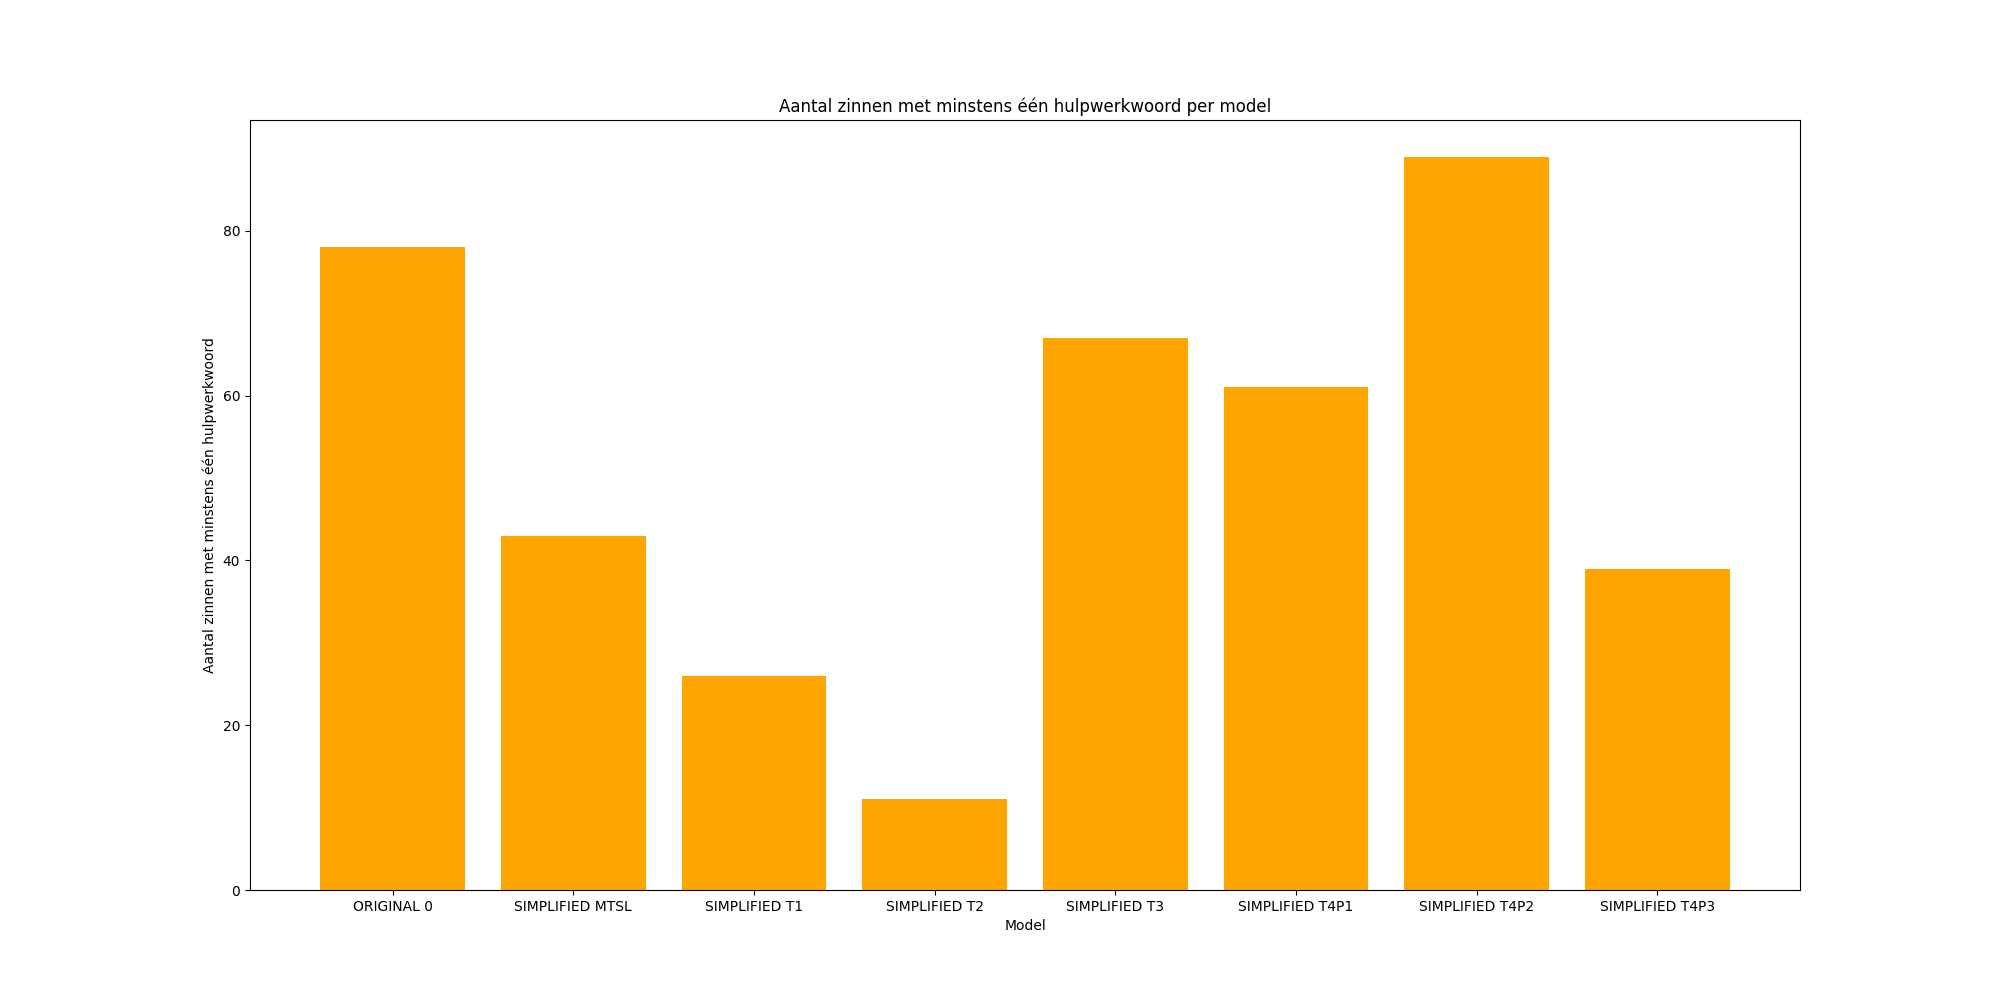
\includegraphics[width=\linewidth]{img/boxplot-aux-a1.png}
	\caption{Gemiddeld aantal lange woorden per zin gegroepeerd op model.}
	\label{img:histplot-aux-a1}
\end{figure}

\begin{figure}
	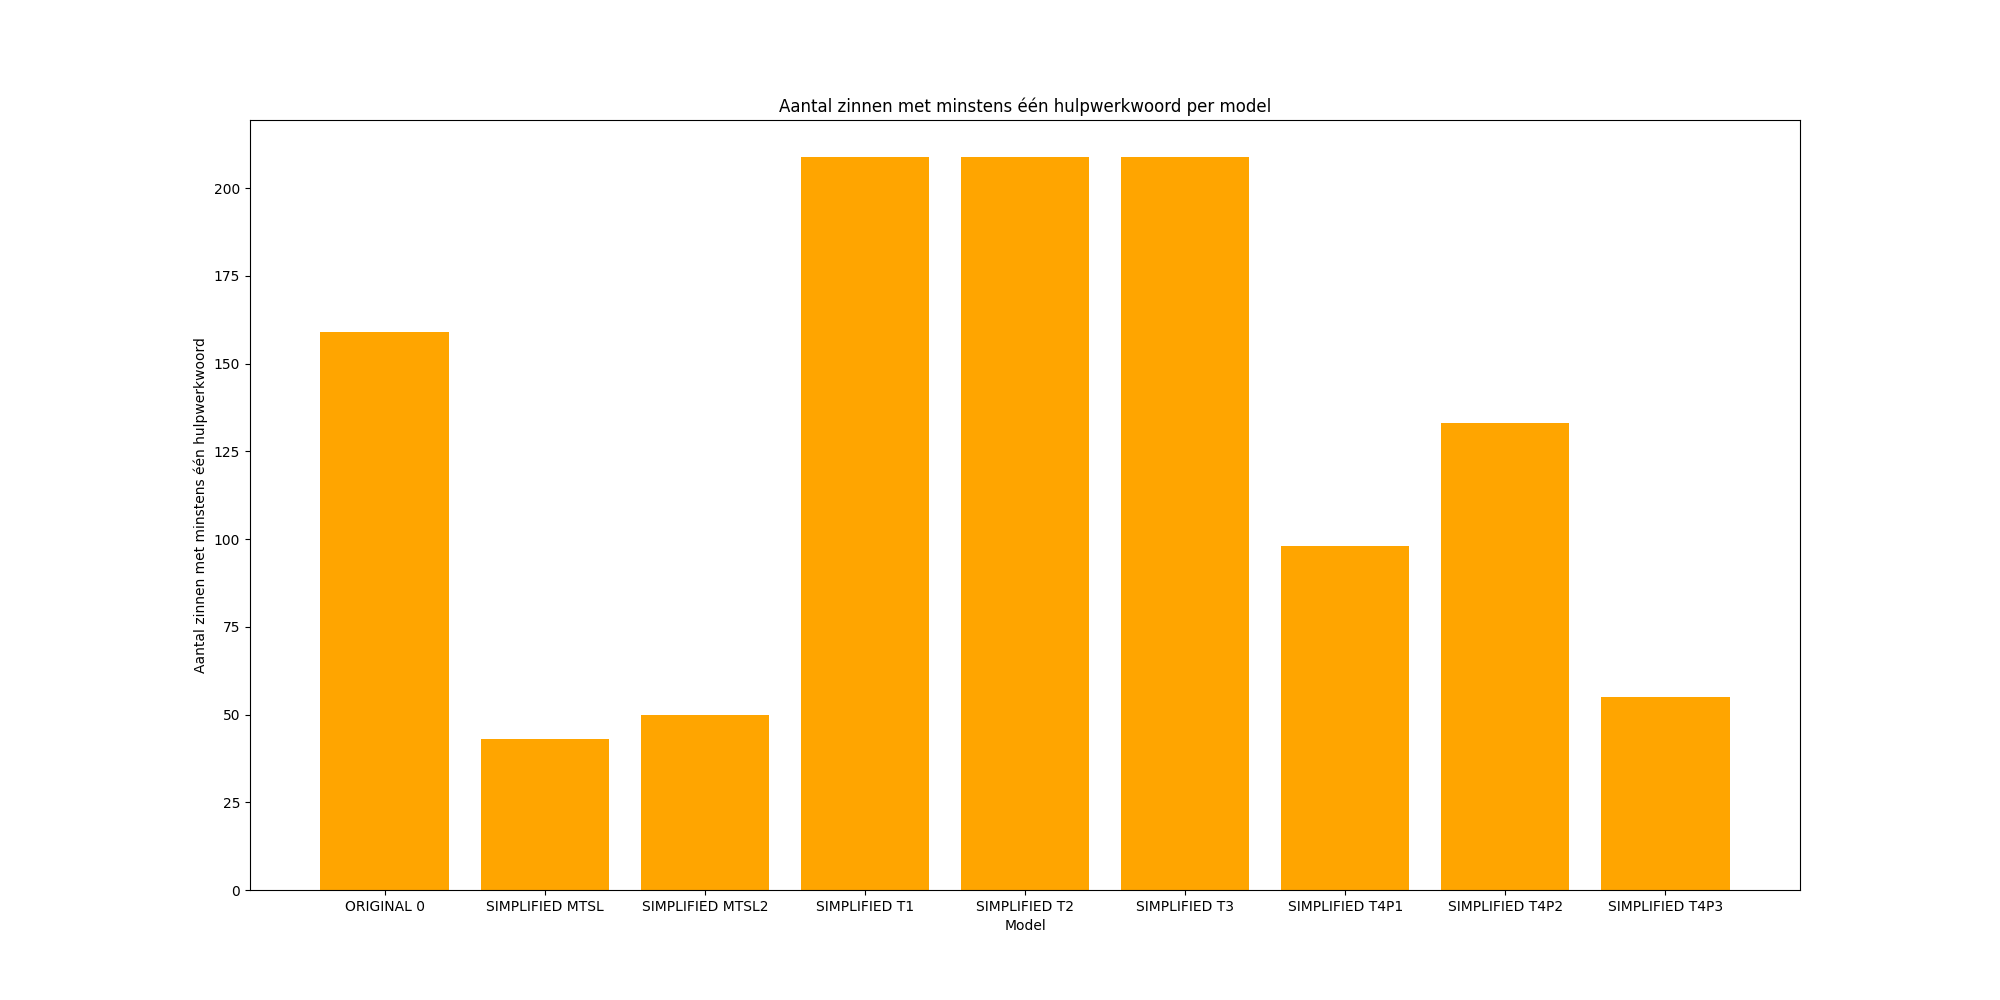
\includegraphics[width=\linewidth]{img/boxplot-aux-a2.png}
	\caption{Gemiddeld aantal lange woorden per zin gegroepeerd op model.}
	\label{img:histplot-aux-a2}
\end{figure}

% tobe

\begin{figure}
	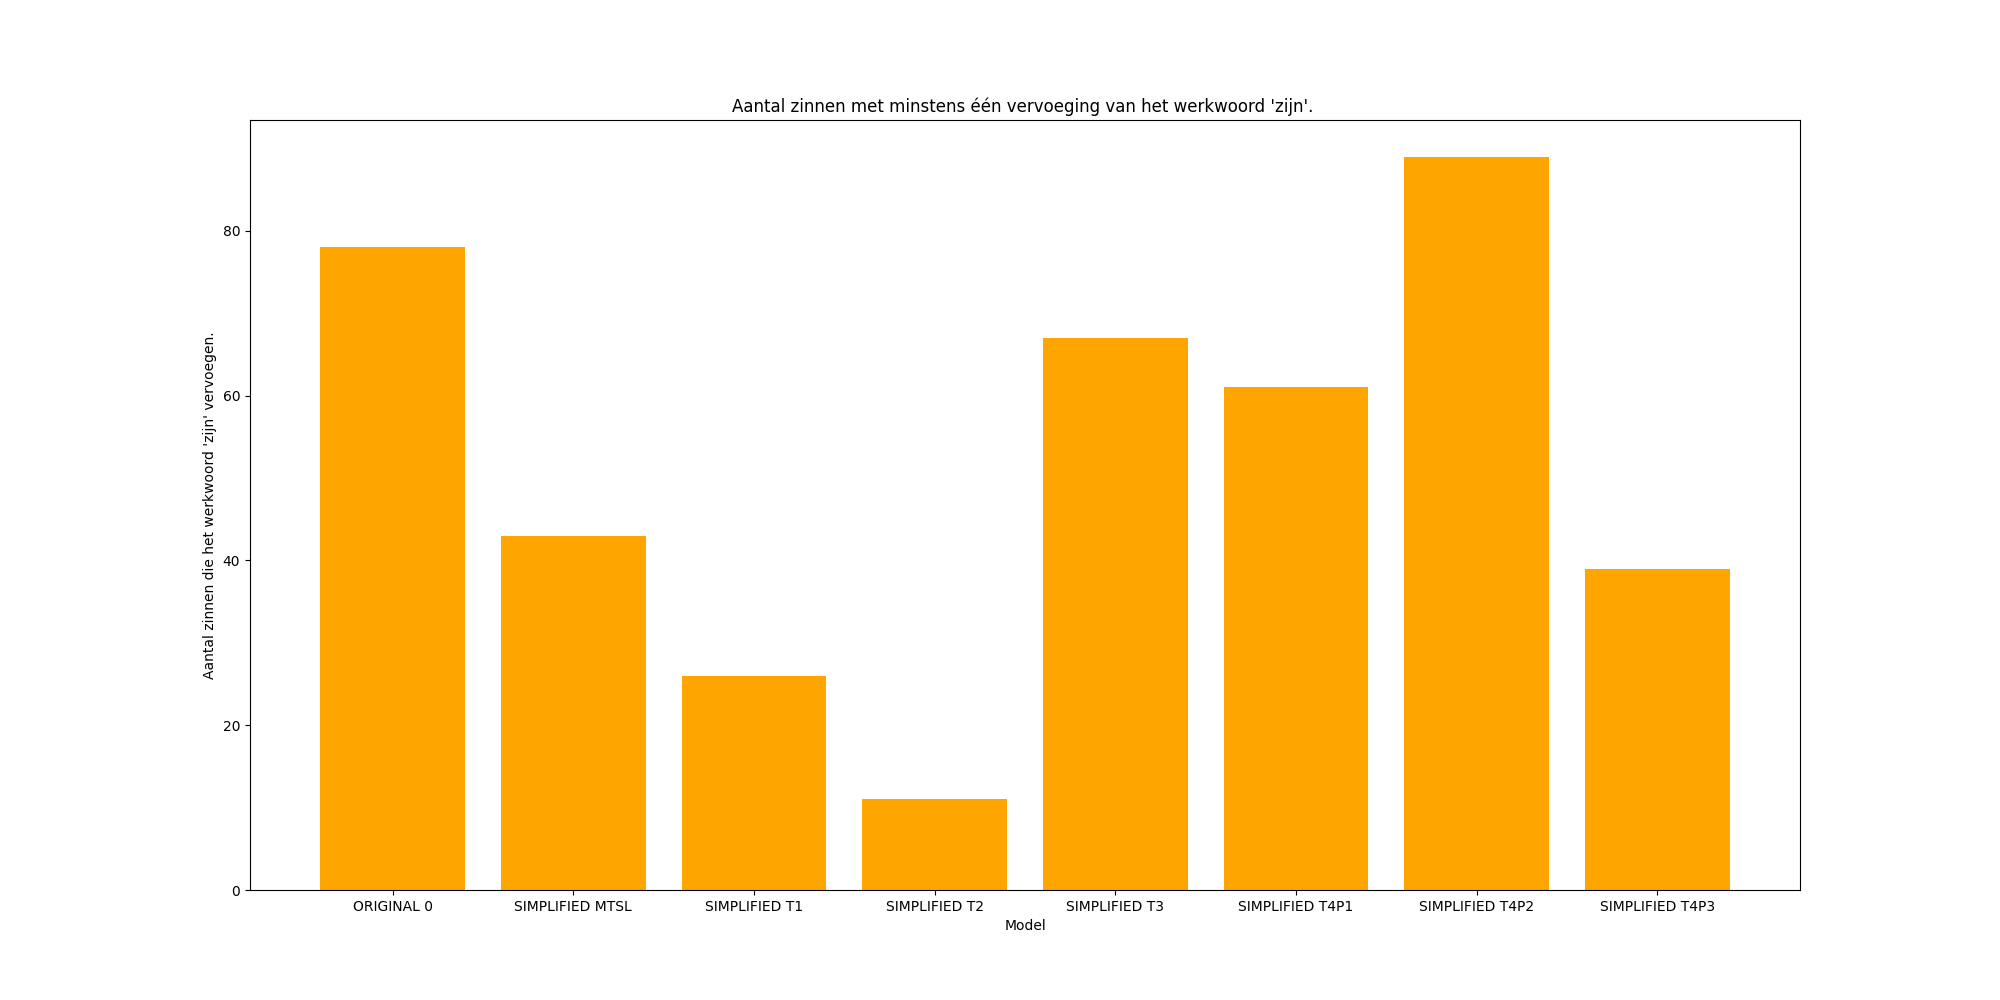
\includegraphics[width=\linewidth]{img/boxplot-tobe-a1.png}
	\caption{Gemiddeld aantal lange woorden per zin gegroepeerd op model.}
	\label{img:histplot-tobe-a1}
\end{figure}

\begin{figure}
	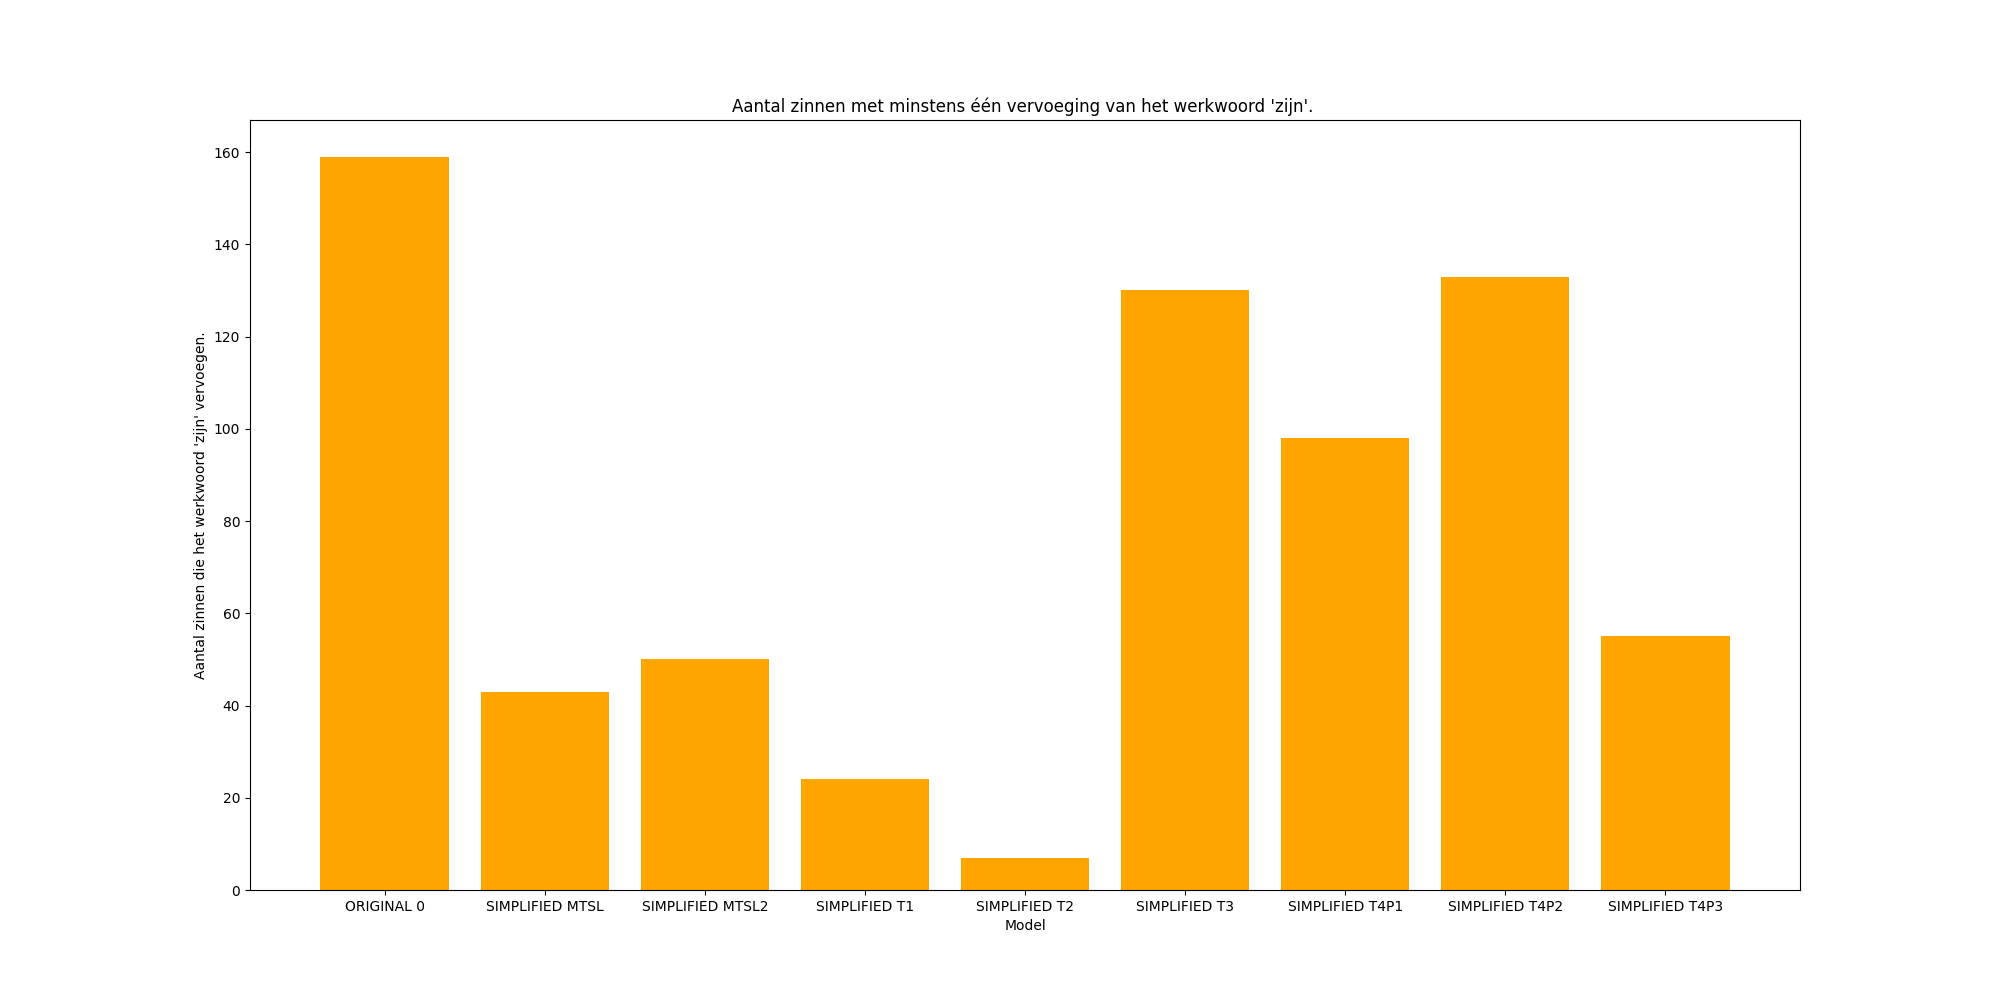
\includegraphics[width=\linewidth]{img/boxplot-tobe-a2.png}
	\caption{Gemiddeld aantal lange woorden per zin gegroepeerd op model.}
	\label{img:histplot-tobe-a2}
\end{figure}


% NB: all readability formulas were developed for English, so the scales of the outcomes are only meaningful for English texts. The Dale-Chall measure uses the original word list for English, but for Dutch and German lists of frequent words are used that were not specifically selected for recognizability by school children.


\subsubsection{Beoordeling op basis van referentieteksten en capaciteiten}

Taalmodellen T1, T2, T3 bieden geen opties voor gepersonaliseerde tekstvereenvoudiging. 

T1, T2 en T3 zijn niet in staat om syntactische vereenvoudiging op een tekst toe te passen. T3 is bij alle prompts in staat om de syntax van een zin te verlagen. Alle uitgeteste taalmodellen zijn echter wel in staat om lexicale vereenvoudiging te realiseren, al wordt de inschatting van de doelgroep in twijfel getrokken. De referentieteksten schatten de doelgroep correct in, door reeds gekend jargon niet aan te passen, maar nieuwe jargon wel aan te passen naargelang er een beschikbaar synoniem is. 

\medspace

De modellen T1, T2 en T3 zijn niet in staat om syntactische vereenvoudiging op een tekst toe te passen. Alleen T4 kan via de prompts P2, P3, P4, P5 en P6 de zinsstructuur verlagen. Hoewel alle geteste taalmodellen in staat zijn om lexicale vereenvoudiging te realiseren, wordt de nauwkeurigheid van de doelgroepsinschatting in twijfel getrokken. De referentieteksten schatten de doelgroep correct in door bekend jargon niet aan te passen, maar wel nieuwe jargon aan te passen als er een beschikbaar synoniem is.  Daarnaast kan T3-P1 ook de coherentie van een meegegeven paragraaf bevorderen, door onder meer omslachtige zinsstructuren aan te passen naar signaalwoorden. In tegenstelling tot GPT-3 zijn de modellen T1, T2 en T3 niet in staat om het formaat van de uitvoer aan te passen. De uitvoer blijft een doorlopende tekst. In de referentietekst past één van de auteurs het formaat aan naar tabelvorm voor enkele paragrafen, waar de inhoud beter in tabelvorm kan gestructureerd worden. Enkel prompts P5 en P6 wordt er expliciet gevraagd om een formaatwijziging, anders geeft T4 vrijwel altijd een doorlopende tekst terug. Zonder de expliciete aanduiding is het model niet in staat om dit zelf te bepalen. Verder onderzoek moet uitwijzen of T4 in staat is om zelfstandig deze bepaling kan maken, zo niet kan deze formaatwijziging niet automatisch bepaald worden en is er tussenkomst van de eindgebruiker vereist. Dit moet ook zo opgenomen worden als een functionaliteit in het prototype. Het formaat van de uitvoer bij de modellen T1, T2 en T3 zijn identiek aan dat van de oorspronkelijke tekst, namelijk in de vorm van een doorlopende tekst. Deze twee modellen zijn niet in staat om het voorbeeld van één van de auteurs te volgen, door formaatwijzigingen toe te passen. Eerder wees de requirementsanalyse uit dat T4 in staat is om met een expliciete prompt het formaat van de tekst aan te passen.

\medspace

De \textit{execution time} van T1 en T2 per API kan oplopen tot hoogstens 30 seconden voor een zin van tien tot dertig woorden, vergeleken met T3 die dezelfde zin in minder dan 10 seconden kan vereenvoudigen.

\medspace

% TODO NIET HIER
% Ontwikkelaars hebben toegang tot T1, T2 en T3 via HuggingFace voor lexicale vereenvoudigingstaken. Deze taalmodellen zijn echter ontoereikend voor gepersonaliseerde tekstvereenvoudiging en daarom is T4 een geschikter model voor het vereenvoudigen van wetenschappelijke artikelen op maat. GPT-3 presteert goed op gepersonaliseerde vereenvoudigingstaken, maar het is belangrijk om op te merken dat geen enkel taalmodel de doelgroep altijd nauwkeurig kan inschatten. Extra trainingsdata, zoals leerstof of wetenschappelijke artikelen die wel op het niveau van een 16-18-jarige is geschreven, kan het model steunen bij de doelgroepsinschatting. Het gebruik van Engelstalige prompts waarin expliciet de gewenste uitvoertaal wordt vermeld, resulteert in coherentere teksten dan bij een Nederlandstalige prompt.

\section{Opbouw van het prototype}

Het prototype voldoet aan alle functionaliteiten die zijn gespecificeerd in het Moscow-schema \ref{img:moscow}. Het overtreft daarmee elke andere tool uit de requirementsanalyse op alle gebieden. Het is vooral op het gebied van formaatwijzigingen de beste, wat suggereert dat het prototype de huidige staat van deze toepassingen weergeeft, gezien de consistente ontwikkeling van de personalisatieopties. Op het gebied van tekstvereenvoudiging scoort het prototype vergelijkbaar of iets beter dan wat GPT-3 kan, wat voor zich spreekt aangezien het twee identieke taalmodellen zijn.

\medspace

Ontwikkelaars kunnen de opgebouwde flowchart volgen om team van vier rollen, namelijk systeem, data, NLP en web ontwikkelaars, te begeleiden doorheen de ontwikkeling van een toepassing voor tekstvereenvoudiging. De flowchart benadrukt dat deze handelingen ook perfect parallel kunnen worden uitgevoerd. Jupyter notebooks bieden een ontwikkelaarsvriendelijke manier om de code vooraf met eenduidige visuele feedback te kunnen testen.

\medspace

Dit prototype maakt geen gebruik van lokaal gehoste taalmodellen. Zo vermindert de nodige rekenkracht en geheugenruimte op het systeem waarop het prototype draait in vergelijking met een lokaal gehost taalmodel. Wanneer ontwikkelaars de toepassing willen uitrollen naar het grote publiek, kunnen ze overschakelen naar lokaal gehoste taalmodellen in plaats van taalmodellen per API. Door de taalmodellen verder te finetunen en te trainen op meer datasets, kunnen AI-ontwikkelaars betere resultaten behalen. 

\medspace

Het ontwikkelen van gebruikersvriendelijke handelingen kan gemakkelijk en snel worden ontwikkeld met behulp van HTML, CSS en JavaScript, zonder de nood van een complex framework. Uit onderzoek blijkt echter dat deze methoden eenvoudig te ontwikkelen zijn, zelfs door pas afgestudeerde bachelorstudenten. AI-softwarebedrijven zouden meer moeten inzetten op personalisatie-opties voor scholieren met dyslexie in de derde graad van het middelbaar onderwijs, omdat zij momenteel het meest betrokken zijn bij de digitalisering. Later kunnen softwareontwikkelaars overgaan op een complexer of robuuster framework. Verder onderzoek is nodig naar het ideale framework om een gepersonaliseerde weergave mogelijk te maken, aangezien dit momenteel nog wordt gedaan met handmatige JavaScript-functies. Een front-end framework dat dit alles beheert, zou handiger zijn voor webontwikkelaars.

\medspace

Dit prototype is momenteel alleen beschikbaar in een lokale omgeving en kan nog niet worden gebruikt door het grote publiek. Het prototype kan teksten lexicaal en syntactisch vereenvoudigen wanneer deze in PDF- of volledige tekstformaat worden ingevoerd. Het prototype heeft functionaliteit voor zowel docenten als studenten, die elk verschillende prioriteiten hebben. Hoewel testen nog nodig zijn, wordt dit wel aangeraden. Onderzoekers op het gebied van logopedie kunnen het prototype testen bij studenten met dyslexie na een (begeleide) installatie van de vereiste set-up. Ook onderzoekers op het gebied van onderwijs kunnen dit gebruiken om de meningen van zowel studenten als docenten te verzamelen en zo de effectiviteit van het prototype te beoordelen. Deze experimenten zijn belangrijk omdat ze kunnen wijzen op de effectiviteit van het prototype.

